%%%%%%%%%%%%%%%%%%%%%%%%%%%%%%%%%%%%%%%%%%%%%%%%%%%%%%%%%%%%
\documentclass[a4paper,11pt,oneside]{article}
\usepackage[a4paper,vmargin={1.5cm,1.5cm},width=17cm]{geometry}
\usepackage[style=verbose-inote,doi=false,sortcites=true,block=space]{biblatex}
\usepackage[utf8]{inputenc}
\usepackage{textcomp}
\usepackage[spanish]{babel}
\usepackage{microtype}
\usepackage{lmodern}
\usepackage{graphicx}
\usepackage{fancyhdr}
\usepackage{booktabs}
\usepackage{eurosym}
\usepackage{hyperref}

%%%%%%%%%%%%%%%%%%%%%%%%%%%%%%%%%%%%%%%%%%%%%%%%%%%%%%%%%%%%
%% HEADERS
\setlength{\headheight}{1cm}
\setlength{\headsep}{0.5cm}
\pagestyle{fancyplain}
\fancyhf{}
\lhead{\fancyplain{}{\sc Memoria científico técnica de proyectos coordinados}}
\rhead{\fancyplain{}{\sc NEXT}}
\cfoot{\thepage}
\renewcommand{\headrulewidth}{0pt} % remove lines
\renewcommand{\footrulewidth}{0pt}

%%%%%%%%%%%%%%%%%%%%%%%%%%%%%%%%%%%%%%%%%%%%%%%%%%%%%%%%%%%%
%% Hack to make math formulas bold in section titles
\makeatletter
\DeclareRobustCommand*{\bfseries}{%
  \not@math@alphabet\bfseries\mathbf
  \fontseries\bfdefault\selectfont
  \boldmath
}
\makeatother

%%%%%%%%%%%%%%%%%%%%%%%%%%%%%%%%%%%%%%%%%%%%%%%%%%%%%%%%%%%%
\def\thesection{\bf \textsf{\alph{section}}}

%\nobibliography{biblio}
%\bibliographystyle{JHEP}

\bibliography{biblio}


%%%%%%%%%%%%%%%%%%%%%%%%%%%%%%%%%%%%%%%%%%%%%%%%%%%%%%%%%%%%
\begin{document}

%% Some useful definitions
\input{src/Commands.tex}

%% Heading
\begin{center}
{\Large \textsf{Convocatorias 2014}} \\ \vspace{0.3cm}
{\Large  \textsf{Proyectos de I+D ``Excelencia'' y Proyectos de I+D+I ``Retos Investigación"}} \\ 
{\Large \textsf{Dirección General de Investigación Científica y Técnica}} \\
{\Large \textsf{Subdirección General de Proyectos de Investigación }} \\ 
%\vspace{0.5cm}
%{\LARGE \bf \textsf{Construcción puesta a punto y operación del experimento NEXT en el Laboratorio Subterráneo de Canfranc} }\\ 
%\vspace{0.3cm}
%{\LARGE \bf \textsf{Construction, commissioning and operation of the NEXT experiment at the Canfranc Underground Laboratory }}\\ 
\end{center}


\section{\bf \textsf{RESUMEN DE LA PROPUESTA/SUMMARY OF THE PROPOSAL}}
\subsection{\sc DATOS DEL PROYECTO COORDINADO}

{\sc INVESTIGADOR COORDINADOR PRINCIPAL:} Ju\'an Jos\'e  G\'omez-Cadenas
\vspace{0.3cm}

{\sc TÍTULO GENERAL DEL PROYECTO COORDINADO:} Construcci\'on, instalaci\'on y operaci\'on del experimento NEXT en el Laboratorio Subterraneo de Canfranc

\vspace{0.3cm}

{\sc ACRÓNIMO DEL PROYECTO COORDINADO:} NEXT.
\vspace{0.3cm}

{\bf RESUMEN DEL PROYECTO COORDINADO:} 
\vspace{0.3cm}
%%%

NEXT (Neutrino Experiment with a Xenon TPC) es un experimento para buscar desintegraciones doble beta sin neutrinos (\bbonu), cuya detección demostraría unívocamente que el neutrino es una partícula de Majorana (es decir su propia antipartícula) y supondría un descubrimiento con profundas consecuencias en física de partículas y cosmología. 

La primera fase de NEXT ha sido completada con éxito. Durante esta etapa el grupo del IFIC ha construido el prototipo NEXT-DEMO que opera en nuestro laboratorio desde 2011 y ha sido esencial para  demostrar las características principales de la tecnología, a saber: excelente resolución de energía y caracterización de la señal mediante la reconstrucción de las trayectorias de los dos electrones emitidos en la desintegración \bbonu. 

Este  proyecto requiere financiación para demostrar una nueva idea que aumentaría dramáticamente las posibilidades de realizar un descubrimiento y situaría a NEXT como el líder mundial del campo. Concretamente se propone añadir un campo magnético al experimento, capaz de aportar una caracterización adicional a la señal, ya que las trayectorias de los dos electrones emitidos en el proceso \bbonu\ se curvarían siguiendo una doble hélice. Para demostrar experimentalmente esta señal, se propone operar NEXT-DEMO en un imán solenoidal (TPC90) disponible en el CERN.

Este proyecto propone también la demostración de un avance radical en tecnología: el uso de sensores de estado sólido (SiPMs) de bajo ruido y capaces de funcionar en campo magnético, y que reemplazarían a los fotomultiplicadores con los que NEXT-DEMO mide la energía de los sucesos. Este desarrollo tendría inmediatas aplicaciones a la técnica PET-MRI que combina tomografía de electrón-positrón con resonancia magnética y necesita, por tanto, cubrir amplias áreas con sensores de bajo ruido capaces de operar en campo magnético.   

 
 \vspace{0.3cm}

{\sc PALABRAS CLAVE DEL PROYECTO COORDINADO:} neutrinos, TPC, HPXe, xenón, desintegración doble beta, Canfranc, alta presión, electroluminescencia. 

 \vspace{0.6cm}
{\sc TITLE OF THE COORDINATED PROJECT:} Construction commissioning and operation of the NEXT experiment at the LSC underground laboratory. 
\vspace{0.3cm}

{\sc ACRONYM OF THE COORDINATED PROJECT:} NEXT.
\vspace{0.3cm}

{\bf SUMMARY OF THE COORDINATED PROJECT:} 
\vspace{0.3cm}

%NEXT (Neutrino Experiment with a Xenon TPC) is an experiment to search for neutrinoless double beta decay events. Detecting such events would be a major discovery that would demonstrate that the neutrino is a Majorana particle (that is, its own antiparticle). 

The first phase of NEXT has been completed successfully. During this period the IFIC group has built the prototype NEXT-DEMO, which operates in our laboratory since 2011 and has been essential to demonstrate the main features of the technology, namely: excellent energy resolution and characterization of the signal by means of the reconstruction of the trajectories of the two electrons emitted in the \bbonu\ decay.

This project requires funding to demonstrate a new idea that would boost dramatically the potential to make a discovery and would place NEXT as the World leader for the field. Specifically we propose to add a magnetic field to the experiment, capable to bring in an additional characterization to the signal, since the trajectories of the two electrons emitted in the \bbonu\ decay would follow a double helix. To demonstrate experimentally this signal, we propose to operate NEXT-DEMO in a solenoid magnet (TPC90) available at CERN.

This project proposes also the demonstration of a radical advance in technology: the use of solid state sensors (SiPMs) of low noise capable to operate in a magnetic field. The SiPMs would replace the PMTs that NEXT-DEMO uses to measure the energy of the events. This development would have immediate applications to the PET-MRI technology where electron-positron tomography is combined with magnetic resonance imaging. PET-MRI devices need to cover large areas with low-noise sensors capable to operate in a magnetic field, such as the SiPMs that we propose to use for this project

 \vspace{0.3cm}

{\bf KEYWORDS OF THE COORDINATED PROJECT:} neutrinos, TPC, HPXe, xenon, double beta decay, Canfranc, high pressure electroluminescence. 

\section{INFORMACIÓN ESPECÍFICA DEL EQUIPO}

% Los objetivos específicos de cada uno de los subproyectos participantes, enumerándolos brevemente, con claridad, precisión y de manera realista (acorde con la duración prevista del proyecto).
%
% En los subproyectos con dos investigadores principales, deberá indicarse expresamente de qué objetivos específicos se hará responsable cada uno de ellos.
%

\subsubsection*{USC team members}

%Members of the USC team:

\begin{enumerate}

\item {\bf Jos\'e \'Angel Hernando Morata} \\ Profesor Titular de Universidad desde Julio 2000 \\
 Departamento de F\'isica de Part\'iculas \\
 Universidade de Santiago de Compostela

\item {\bf Gonzalo Mart\'inez Lema} \\ 
Master en F\'isica de Part\'iculas.  \\
Contratado como graduado universitario dentro del  proyecto ``Canfranc Underground Physics", Consolider CSD2008-00037. 

\end{enumerate}


% Los objetivos específicos de cada uno de los subproyectos participantes, enumerándolos brevemente, con claridad, precisión y de manera realista (acorde con la duración prevista del proyecto).
%
% En los subproyectos con dos investigadores principales, deberá indicarse expresamente de qué objetivos específicos se hará responsable cada uno de ellos.
%

\subsubsection*{USC previous projects}

These are the projects that the IP, Jose A. Hernando, has participated in:

\begin{enumerate}

\item Title: ``Medidas de precisi\'on en F\'isica del sabor en el LHCb". \\
Ref:  FPA2011-23608, Ministerio de Econom\'ia y Competitividad \\
Budget: 563.000 \euro \\
IP: Bernardo Adeva Andany \\
Institution: Universidade de Santiago de Compostela \\
Period: 01/2012-12/2014

\item Title: ``Canfranc Underground Physics (CUP)"\\
Ref:  CSD2008-00037, Ministerio de Educaci\'on y Ciencia \\
Budget: 5.000.000 \euro \\
IP: Mar\'ia Concepci\'on Gonz\'alez-Garc\'ia \\
Institution: Universitat de Barcelona \\
Period: 01/2009-12/2014

\item Title: ``Contribuci\'on a la reconstrucci\'on de trayectorias y al sistema de disparo de alto nivel del experiment LHCb" \\
Ref:  FPA2007-65268, Ministerio de Educaci\'on y Ciencia \\
Budget:  190.000 \euro \\
IP: Jose Angel Hernando Morata \\ 
Institution: Universidade de Santiago de Compostela \\
Period: 01/2009-12/2009

\end{enumerate}


\section{\bf DOCUMENTO CIENTÍFICO/SCIENTIFIC DOCUMENT}

\subsection{\sc JUSTIFICACIÓN DE LA COORDINACIÓN/JUSTIFICATION OF THE COORDINATION}
\vspace{0.3cm}

%NEXT is organised as an international collaboration, which includes groups from Spain, Portugal, Russia, US, and Colombia. The spanish groups participating in NEXT are: Instituto de Física Corpuscular (IFIC), a joined center of the University of Valencia (UV) and the Spanish Council for Research (CSIC).The  Polytechnic University of Valencia (UPV). University of Santiago de Compostela (US). Autonomic University of Madrid (UAM); and University of Zaragoza (UZ). 

The leading groups participating in this coordinated project form the core of the collaboration. The spokesperson (and PI of this coordinated project), the technical coordinator, the software coordinator and the leaders of several working  packages are members of IFIC. The coordinators of the electronics, DAQ, and risk management are members of the UPV. The coordinator of calibration and reconstruction is a member of US. The groups participating in this coordinated project invest 100\% of their research time and resources in the NEXT project. 

Another key task for the experiment is that of radio purity, coordinated by the UAM (prof. Luis Labarga) who also presents an project to this call. The project of prof. Labarga includes a proposal to participate in the Super Kamiokande experiment, and for this reason we have considered more appropriated to present separated proposals. The task of radio purity and the corresponding request for resources is described in his project.

%The IFIC, UPV, UV and US groups work in a fully co-ordinated way. The NEXT collaboration is organised in terms of Working Packages (WP) which include members of the different groups. In addition of the WP structure, a general ``hardware coordination meeting'' and a ``software coordination meeting'' which involves members of all the groups is organised on a weekly-basis. Last, but not least, the coordination of the groups is essential to construct, commission and operate the NEW and NEXT-100 detectors at the LSC. The management of the laboratory and its Scientific Committee (SC), require a formal Project Management Plan (PMP) from the NEXT collaboration, and reviews its progress every six months. The PMP integrates the activities of all the collaboration groups and in particular of the groups participating in this project. 

Furthermore, a strong collaboration is currently being formed between IFIC and the Center for Pulsed Lasers (CLPU after the initials of the center in spanish), to develop the laser technology which could be used to tag the barium ion emitted in the \bb\ decays, resulting (when combined with the excellent energy resolution of NEXT and its topological signature) in a virtually background-free experiment. We are in the process of preparing a ``white paper'' detailing the theoretical grounds and the experimental procedures to address a successful  \BATA\ program. 


\subsection{\bf PROPUESTA CIENTÍFICA/SCIENTIFIC PROPOSAL}

%\input{src/CALREC/motivation.tex}

\subsection*{\sc Antecedentes/Previous work}

%\input{src/CALIB/previouswork.tex}

\subsection*{\sc Objetivos/Objectives}

%% Los objetivos específicos de cada uno de los subproyectos participantes, enumerándolos brevemente, con claridad, precisión y de manera realista (acorde con la duración prevista del proyecto).
%
% En los subproyectos con dos investigadores principales, deberá indicarse expresamente de qué objetivos específicos se hará responsable cada uno de ellos.
%

\subsubsection*{Objectives of the CALREC subproject}

The subproject CALREC, under the responsibility of the USC, will provide the calibration systems for the NEW and NEXT-100 detectors (WP14).
In addition the USC group will develop tracking reconstruction algorithms for NEXT, will
take a leading role in the analysis of the NEW and NEXT-100 data (WP13) and will collaborate  in the R+D tasks for BEXT and NEXT 1 ton. 

The different parts of this subproject are:
\begin{enumerate}
\item {\bf Design, construction, commissioning and operation of a calibration system to estimate the gain and noise of the SiPMs and PMTs sensors}. Two sets of 400 nm LEDs will be located on the tracking a energy plane. They will illuminate periodically the detector with a dim light. The gain and noise of SiPMs and PMTs will be estimated from single photo-electron signals (see \cite{NEXT-DEMO}).

\item {\bf Design, construction, commissioning and operation of an energy calibration system with external radioactive sources for NEW and NEXT-100}.
The energy scale and energy resolution in the region of \Qbb ~can be estimated using the photo-peak of the 2.6 MeV gamma from a \Tl~  source. In addition, the photo-peak electron and the two electrons of the double-scape peak (~1.6 MeV) can be used to measure the misidentification efficiency and the signal selection efficiency respectively. With additional 
\NA,  \CS~ sources we can calibrate the energy scale in the range of 500 keV.

\item {\bf Design, construction, commissioning and operation of a position calibration system with X-rays}. X-rays from \Xe~ (30 keV) and \KR ~(42 keV) are point-like sources in NEXT.
They will be used to correct the bias on the energy introduced by geometrical effects and to estimate the light collection at the SiPMs from a point-like source (PSF function). This is a fundamental element for the tracking reconstruction algorithms. R+D will be needed to understand the operation with \KR.

\item {\bf Design, implementation and validation of the tracking reconstruction algorithms of NEXT}.  
They will be validated with MC simulations and the data from the \NA, \CS~  and \Tl~  sources.

\item {\bf Take a leading roll in analysis}. Design and do the measurement of the \bb~ spectrum with NEW data, and Design and prepare the search for \bbonu~  for NEXT-100. 
Again, calibration data from the radioactive sources will be crucial to estimate the efficiencies of the analysis.

\item {\bf Contribute to the R+D for NEXT 1 ton} on noble gas detectors with additives (i.e TMVA) that can result in a smaller electron transverse diffusion and open the possibility to detect dark matter (following the preliminary results on \cite{NEXT-DM)}. This work will be done in collaboration with other NEXT institutions (IFIC and UZ) and using existing prototypes and installations.
\end{enumerate}


\subsection*{\sc Adecuación al programa de Retos de la sociedad/ Idoneity to the program of challenges of society  }

%%Si la memoria se presenta a la convocatoria de RETOS INVESTIGACIÓN, deberá identificarse el reto cuyo estudio se pretende abordar y la relevancia social o económica prevista.
%
This research project is presented within the program of ``Challenges of society'', specifically, challenge number 6: {\bf Change and social innovation.}

We argue that this project represents a major innovation in the way that particle physics is conducted in Spain, and thus marks a path to a more productive approach to research.

Particle physics is a clear example of the so-called ``big-science'',
characterised by the need for large budgets, big machines (such as particle accelerators) and large staffs (for example, the number of physicists participating in the ATLAS and CMS experiments is of the order of 6,000). The discovery of the Higgs boson is a quintessential example of such big science, and clearly shows its pros and cons. 

The obvious pro is the major scientific achievement that the discovery represents. It has required the construction and operation of the LHC, one the most impressive scientific machines ever built by humankind. The gargantuan scale of the effort could only be met by a collective effort centralised in the largest particle physics laboratory in the World, CERN.  

Among the cons of big science are the large budgets that it involves, often invested in purchasing equipment to be installed at CERN and in paying scientific staff whose activity also develops at CERN. Such large budgets are often justified in terms of industrial and scientific returns. While those returns certainly exist, it is often not easy to quantify their impact in the countries that finance big science. Furthermore, {\bf returns tend to be larger for countries who are already well developed scientifically}. Specifically, the positions of leadership in the large CERN experiments, and in the CERN scientific and technical divisions, are dominated by countries like Germany, Switzerland, U.K., France and Italy. 

Remarkably, the countries leading the big science at CERN and other laboratories have also developed ``national science'' physics programs. A case of great interest is Italy, a country not very different from Spain, in terms of GDP and social habits. However, the international impact and the returns of physics in Italy is much larger than in Spain. For example, the number of spanish staff members at CERN is 115, to be compared with 275 corresponding to Italy (which has the second largest staff population, after France, who co-hosts the lab). Adding fellows and associates (that is, temporary CERN contracts, often given to scientists), the figures for Spain are 363, to be compared with 1726 for Italy\footnote{\href{http://council.web.cern.ch/council/en/Governance/TREF-PersonnelStatistics2012.pdf}{http://council.web.cern.ch/council/en/Governance/TREF-PersonnelStatistics2012.pdf}}. Several Italians have served as CERN general directors, and have led or are leading the LHC experiments. The next CERN general director (and perhaps the first woman to occupy such position in the history of the lab) may be the ex-spokesperson of ATLAS, the italian physicist Fabiola Gianotti. Moreover, Italy has four Nobel prizes in physics (Marconi, 1909, Fermi, 1938, Segrè 1959, Rubbia 1984), while Spain has none. 

Remarkably Italy also boasts the best underground laboratory of Europe, and one of the best of the world, the LNGS. The lab hosts 20 experiments including three experiments searching for \bbonu\ processes (GERDA, CUORE and COBRA) and two experiments searching for Dark Matter (WARP and XENON). 

Through these experiments, the italian physics{\bf attracts external talent} (some of the best physicists from Europe and USA participate in experiments at LNGS) {\bf and external funding}, complementing the big science at CERN with physics of a smaller scale concerning human resources and budgets. However, such ``local'' physics results in discoveries of great scientific impact (such as the discovery of neutrino oscillations, which has been the result of a world-wide effort involving underground laboratories in Italy, USA, Canada, Russia and Japan). It also allows the training of students and post-docs in experiments where young physicists can make a major impact at all levels, ranging from the construction of the detector to the analysis of the data. Last, but not least, such local science has an important impact in the italian industry and in the appreciation of science by the public in general. 

We argue that, in order to balance and optimise the current big-science effort in Spain, it is necessary to develop the physics at the LSC, in analogy to the italian case. NEXT is the flagship experiment of our national laboratory, and has achieved intentional recognition, as demonstrated by the fact that is a recognised CERN experiment and has obtained an AdG/ERC, {\bf the first grant of this type in the field of particle physics}. 

We, therefore, consider that the NEXT project is a clear example of social innovation, as it has the potential of implementing profound changes in spanish science. As described in this project, NEXT, through its various stages, can hit a major discovery. It will bring international credit and visibility to our science and to the LSC. And it has an important impact both in local industry (through contracts to many national firms, and development of high technology) and in the public perception of science (thorough a very intense activity in public forums including large-circulation cultural magazines such as JotDown, where the PI of this project directs the science section). 

Furthermore, the on-going collaboration with the CLPU further reinforces the above arguments, since the effort involves now a second national scientific installation. In addition, the \BATA\ program implies a major example of inter disciplinarity, and can result in a number of important technological returns (development of infra-red laser technology, which can be applied to molecular fluorescence, among other examples).

We also argue that the project will bring innovation to the industry-science relation in Spain. The experiment uses and develops high technology, involving national firms. As an example, the construction of radio-pure pressure vessel has been partially financed by CEDETI grants, given the potential industrial returns of high-pressure, high-vacuum technology using titanium and titanium-alloys, our materials of choice. A second example, already mentioned, is our project to develop infrared laser technology at the CLPU, an activity with immediate scientific and industrial returns. Lasers in this spectrum are invisible to the human eye and not absorbed by the atmosphere, having them obvious applications in the surveillance industry. At the same time, IR also enhances night vision equipment capabilities by flooding forward positions with invisible light that enhances light gathering performance and increasing the ability to detect objects at greater lengths.

 The NEXT chamber itself is a 3D imaging chamber using large arrays of SiPMs. Both the instrumentation and the reconstruction software has potential applications to medical imaging. 

Finally it is important to remark that, while the usual operation of big-science in Spain implies to finance the participation of our groups in labs like CERN (including the annual CERN quota, the common-fund of the experiments and the contributions to construction and operation of the CERN experiments), the national science that NEXT represents obtains external funding through ERC projects (including the AdG and several H2020 actions currently in progress involving LSC), as well as the contributions of the international collaboration to detector construction and operation (in particular, in the case of NEXT through the USA groups led by Prof. Dave Nygren, the inventor of the technology in which NEXT is based). NEXT also attracts external talent to our country (as the intense collaboration with top USA universities demonstrates). The NEXT group is very international, and several of our post-docs are or have been financed by EC grants (such as the Marie Curie). 

Last but not least, the NEXT experiment, and in particular the collaboration with the CLPU, involves the extensive development of photonics listed as one of the  "Facilitating Essential Technologies".


\subsection*{\sc Objetivos subproyectos/ Objectives of subprojects}

%\subsubsection*{Objectives of this coordinated project and the NEXT Project Management Plan}

The objectives of this coordinated project correspond to the Working Packages described in the NEXT Project Management Plan (PMP)\footnote{PMP document in NEXT web page}. Specifically: 
\begin{itemize}
\item {\bf WP1: PV (Pressure Vessel)}: Construction of the NEW and NEXT-100 pressure vessels. 
\item {\bf WP2: GS (Gas System)}: Installation and commissioning of the Gas System for NEW and NEXT-100 at the LSC. 
\item {\bf WP3:IS (Infrastructures)}: Construction of the infrastructures (working platform, seismic pedestal, lead castle, radon suppression system and clean tent), needed for the operation of NEW/NEXT-100.
\item {\bf WP4: FC (Field Cage)}: Construction of the field cage, light tube, HVFT and EL grids of NEW and NEXT-100.
\item {\bf WP5: EP (Energy plane)}: Construction of the NEW/NEXT-100 energy planes.
\item {\bf WP6: TP (Tracking plane)}: Construction of the NEW/NEXT-100 tracking planes.
\item {\bf WP7: FEE (Front-End electronics)}: Front-End electronics of energy and tracking planes.
\item {\bf WP8: DAQ (Data Acquisition )}: Data  acquisition of the energy and tracking planes.
\item {\bf WP9 ONL (Online) }: Online monitoring for NEW/NEXT-100. 
\item {\bf WP10: SLW (Slow Controls)}: Slow controls of the detectors, gas system and ancillary systems.
\item {\bf WP11: MC (Monte Carlo)}: Monte Carlo simulation of the detector(s) and implementation of the background model. 
\item {\bf WP12: REC (Reconstruction)}: Offline reconstruction of events in NEW/NEXT-100.
\item {\bf WP13: SOF (Software)}: Development and maintenance of software tools (reconstruction and analysis frameworks, release tools, software libraries) and coordination of data and Monte Carlo productions. 
\item {\bf WP14: CAL (Calibration)}: Calibration of the NEW/NEXT-100 with radioactive sources. 
\item {\bf WP15: RAD (Radiopurity)}: Screening, using the LSC facilities, as well as several other techniques, of all the components being used in the  NEW/NEXT-100 detectors. 
\end{itemize}

The COORD subproject addresses the objectives corresponding to WP1 to WP6, WP11 and WP13. The objectives of the ENG subproject are those corresponding to WP7 to WP10. The objectives of the CALREC subproject are those included in WP12 and WP14. Finally, the objectives of the RPUR subproject are those included in WP15.  


%% Los objetivos específicos de cada uno de los subproyectos participantes, enumerándolos brevemente, con claridad, precisión y de manera realista (acorde con la duración prevista del proyecto).
%
% En los subproyectos con dos investigadores principales, deberá indicarse expresamente de qué objetivos específicos se hará responsable cada uno de ellos.
%

\subsubsection*{Objectives of the COORD subproject}

\begin{figure}
\centering
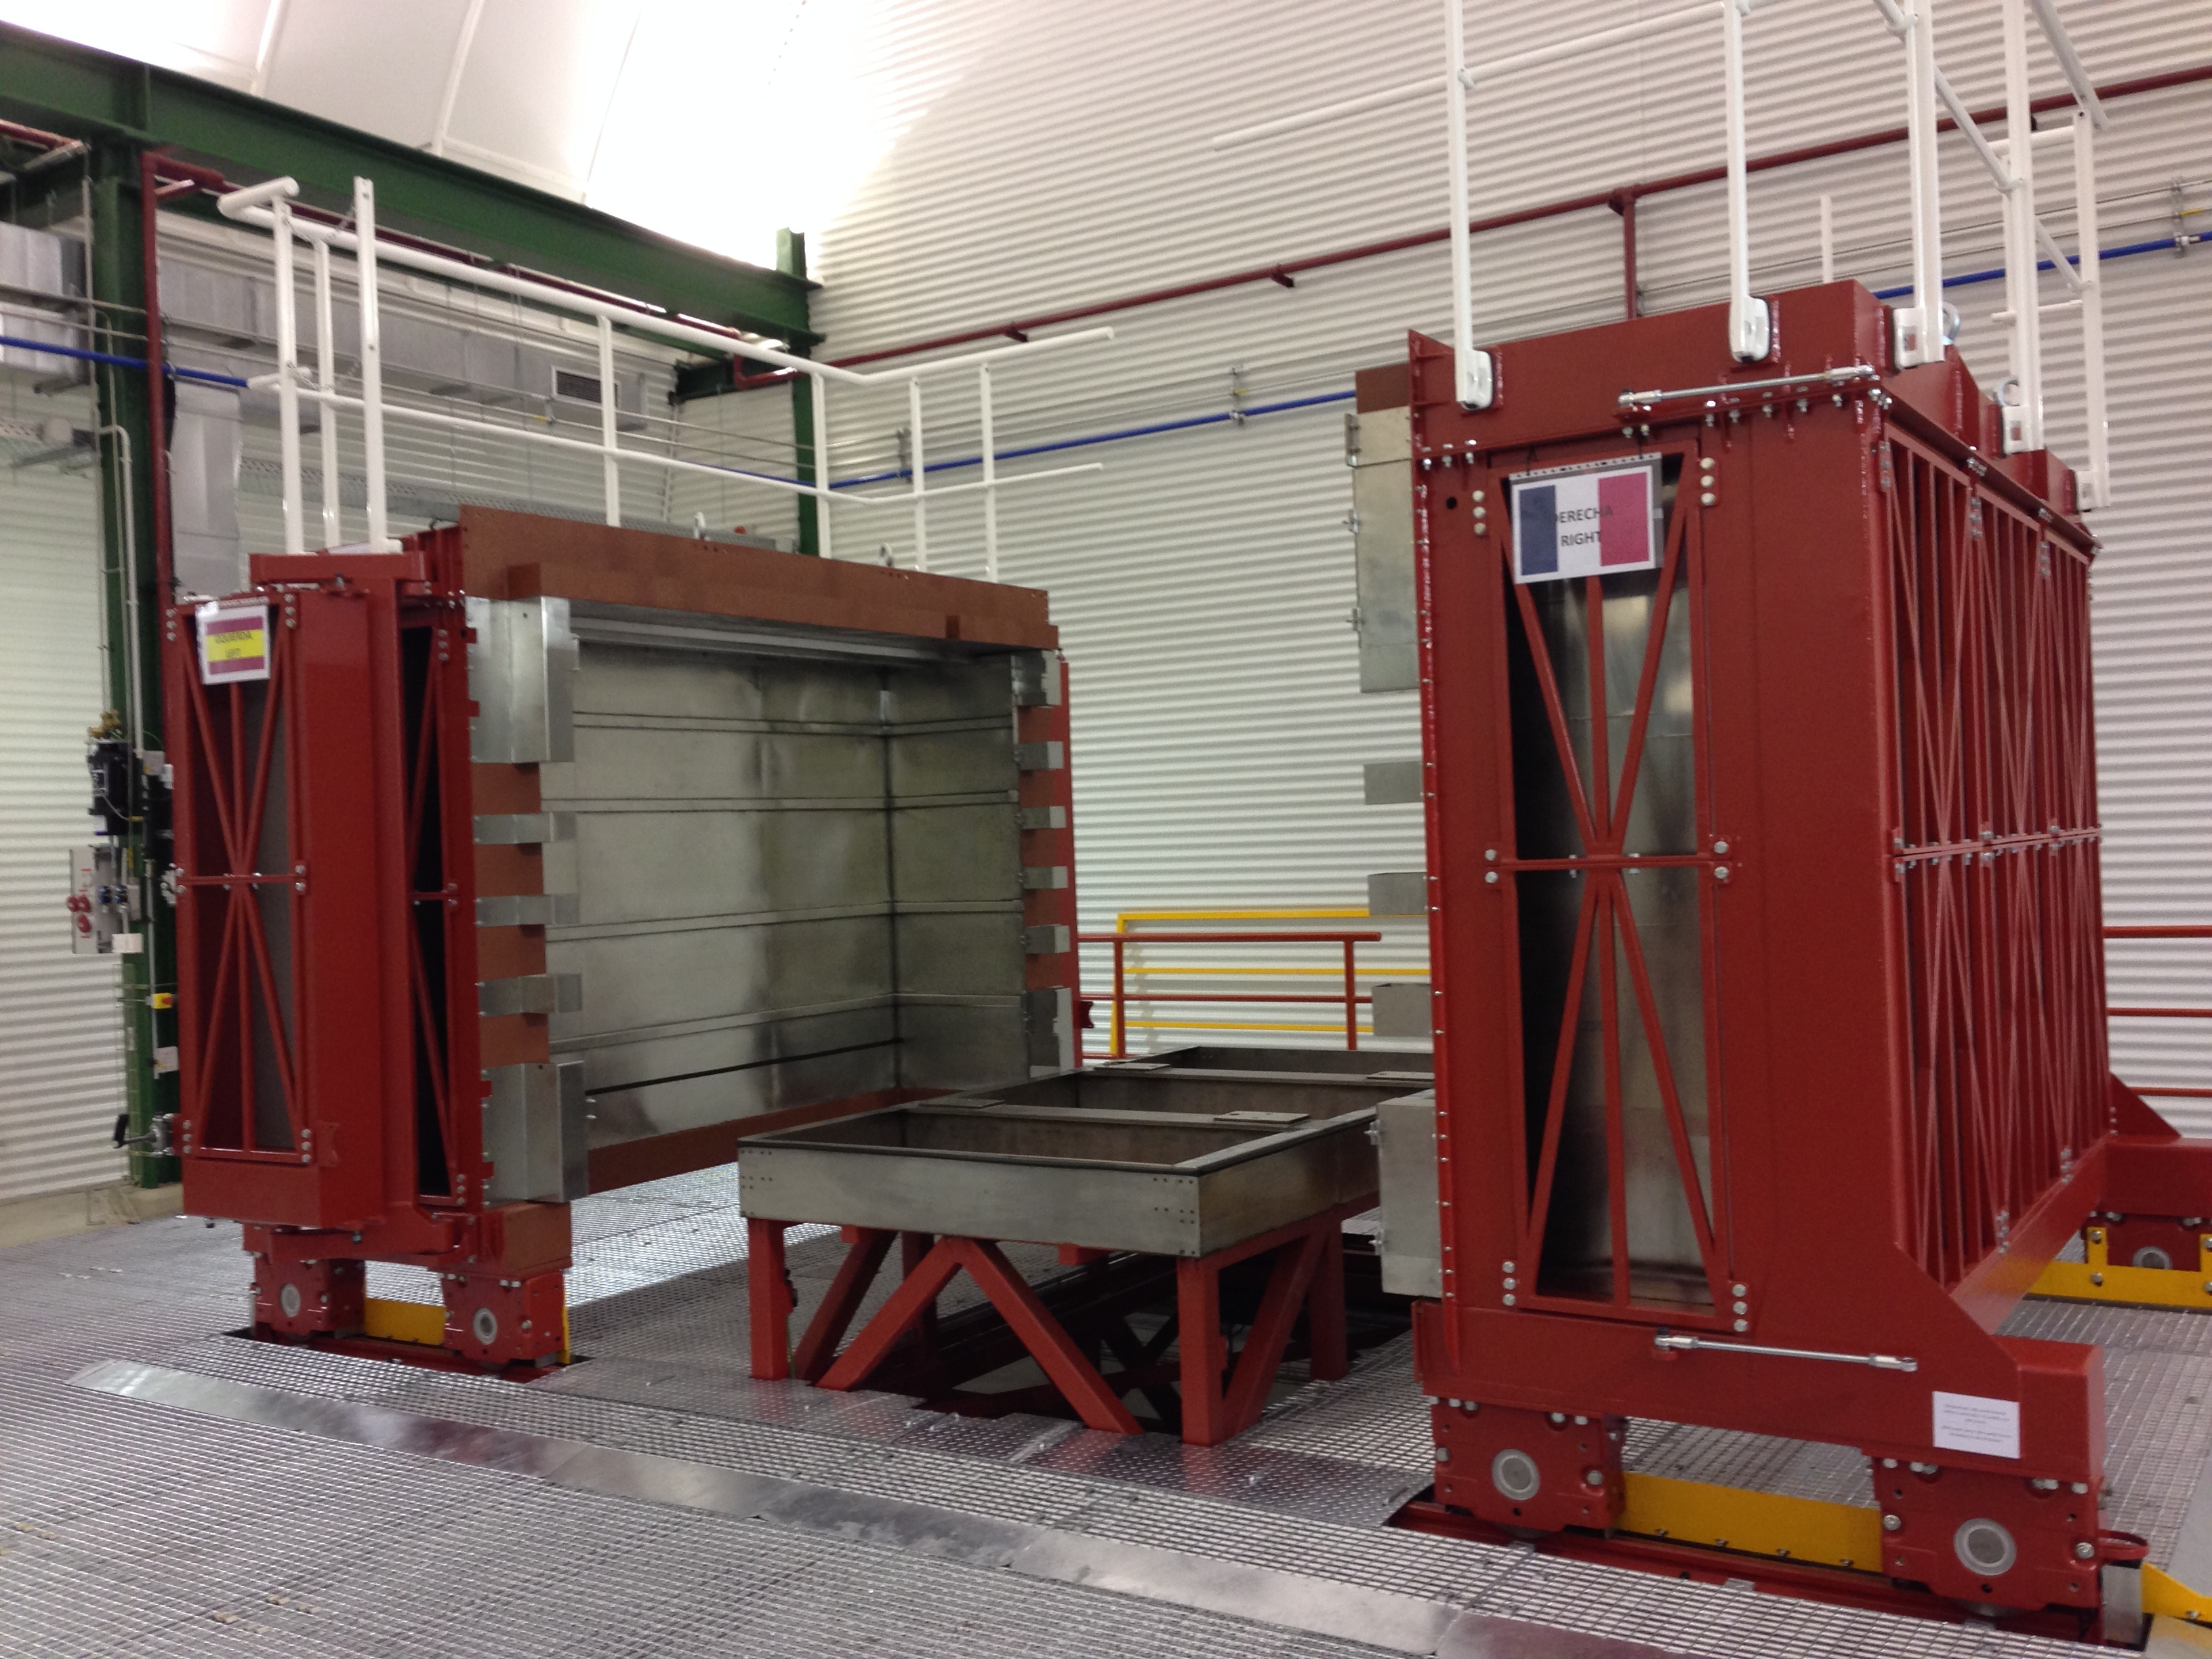
\includegraphics[height=8cm]{img/LeadCastle.jpg}
\caption{The working platform, seismic pedestal and lead castle, in open configuration, at the LSC.} \label{fig:INFRA}
\end{figure}


\begin{figure}
\centering
\includegraphics[height=8cm]{img/PV.png}
\caption{The pressure vessel of NEW (left) and NEXT-100 (right).} \label{fig:PV}
\end{figure}

%%%%%
\begin{figure}[t!b!]
\begin{center}
\includegraphics[width=.9\textwidth]{img/EPNext-100.png}
\end{center}
\caption{Top left: NEXT-100 energy plane (60 PMTs). Top right: NEW energy plane (12 PMTs).
Bottom left: The R11410-10 PMT from Hamamatsu; bottom right: a PMT can prototype.} \label{fig:EnergyPlane}
\end{figure}

%%%%%%%
%\begin{figure}[tbhp!]
%\begin{center}
%\includegraphics[width=0.7\textwidth]{img/TPNext-100.png}
%\end{center}
%\caption{Top left: the tracking plane of NEXT-100, will deploy 107 of the newly developed Kapton Dice Boards (KDB) shown in bottom left (64 SiPM per KDB, no connector, low noise tracing, low radioactivity). Top right: NEW will deploy about 20\% of the KDBs (28). Bottom right: the Cuflon Dice Board containing 16 (4$\times$4) SiPMs used for DEMO. The KDB improves dramatically the technology.} 
%\label{fig.db2}
%\end{figure}
%%%%%%%

The specific objectives of the COORD subproject are:

\begin{enumerate}
\item {\bf Complete the needed infrastructures to operate NEW and NEXT-100 at the LSC}. 
The infrastructures include: a) working platform and seismic pedestal; b) lead castle; c) gas system; d) clean tent; e) radon suppression system. 
\begin{enumerate}
\item The working platform, seismic pedestal and lead castle are already installed at the LSC (Figure \ref{fig:INFRA}).
\item The equipment related with the gas system and emergency recovery system has been purchased during 2014. The gas loop and compressors will be installed at the LSC during the first quarter of 2015 (Q1'15). The emergency recovery system will be installed during the second quarter 2015 (Q2'15). The clean tent and radon suppression system will also be installed during Q2'15. 
\end{enumerate}

\item {\bf Construction of NEW}, foreseen to be completed in Q2'15, and involving:
\begin{enumerate}
\item {\em Construction of the NEW pressure vessel (NPV)}.
The NEW and NEXT-100 pressure vessels, shown in Figure \ref{fig:PV} were designed to withstand pressures in excess of 20 bar, and to operate with negligible losses at 15 bar. They are built using a 316Ti alloy of low activity ($\sim$0.2 mBq/kg for the thorium series and the uranium series, as measured by our screening campaign). 

The design of the PV was a collaboration between IFIC and LBNL groups. They have been manufactured by several Spanish companies (TRINOS, MOVESA and ACYM) and has benefited from a CEDETI grant. Currently (Q4'14) the NEW pressure vessel (NPV) is being fitted with a copper shield (called the Inner Copper Shield, ICS) that attenuates residual ambient radiation. NPV will be shipped tested for functionality at IFIC in Q1'15, then shipped to LSC and commissioned during Q2'15. 

\item {\em Construction of the NEW field cage (NFC)}
The NEW field cage (NFC) produces an uniform electric ($\sim$ 300 V/cm) field inside the  detector that drifts the ionisation electron to the anode, where they are further accelerated in the electric field produced between a pair of transparent grids, called the electroluminescent (EL) grids. 

The main body of the field cage is a high density polyethylene (HDPE) cylindrical shell with a 2.5\,cm wall thickness.  The drift region will consist of radiopure  copper strips connected with low radioactivity resistors.  The light tube consists of thin sheets of teflon, coated with tetraphenyl butadiene (TPB) wavelength shifter to shift the UV light produced in xenon to the blue region (PMT and SiPMs operate best in this region, around 450 nm).  A high-voltage feedthrough (HVFT) in the cathode and another one in the anode, allow the definition of the voltages. The cathode HVFT is designed to withstand up to 100 kV, and the HVFT of the anode to withstand up to 40 kV. The design of the HVFT, identical for NEW and NEXT-100 improve those that were built for DEMO by the Texas A\&M group. The field cage and grids of NEW and NEXT-100 are also identical, to a scale 1:2. The grids use a stainless steel mesh with pitch 0.5 mm and wire diameter 30 microns, which results in an open area of 90\%.  

The construction of NFC is currently under way (Q4' 2014). The HDPE body is being manufactured by the AIMPLAS company. The HVFT and the grids are being manufactured at Texas. The  NFC will be tested at IFIC before shipping to the LSC in Q1'15. Installation and commissioning at the LSC will occur in Q2'15. 

\item {\em Construction of the NEW energy planes (NEP)}
In NEW the energy measurement will be provided by the detection of EL light via PMTs, which will also record the scintillation light needed for $t_0$. Those PMTs will be located behind a transparent cathode.

A total of 12 low-background, high-QE PMTs, model R11410-10 from Hamamatsu covering 32.5\% of the cathode will be deployed. The R11410-10 are large tubes, with a 3'' photocathode and low levels of  activity of the order of 1 mBq per unit in the Uranium and Thorium series. The PMTs are sealed into individual pressure resistant, vacuum tight copper enclosures (called PMT cans) coupled to 
sapphire windows, coated with ITO (for electrical conductivity) and TPB. 

The NEW energy plane (NEP), shown in Figure \ref{fig:EnergyPlane}
is currently (Q4'15) under construction at IFIC. The PMT can design have been validated with prototypes (see Figure  \ref{fig:EnergyPlane}), and production of the parts has started. The NEP will ship to LSC during Q1'15 and commissioned, together with the rest of the detector in Q2'15. 

\item  {\em  Construction of the NEW tracking plane (NTP)}:
In NEW the tracking function is provided by a plane of multi-pixel photon counters (SiPMs) operating as a light-pixels and located behind the transparent EL grids. They are mounted in flexible radiopure Kapton Dice Boards (KDB). Each KDB hosts 64 SiPMs The NTP will deploy 28 such KDBs. 

The NTP is currently under construction at IFIC (Q4'14). The KDB production has been validated and prototypes have demonstrated excellent performance. The NEP will ship to LSC during Q1'15 and commissioned, together with the rest of the detector in Q2'15.  

\end{enumerate}
 
\item {\bf Commissioning of NEW and evaluation of performance}. The NEW detector will be brought online in Q2'15, and extensive testing will be performed to certify safe and stable operation (no leaks, no sparks), as well as testing and integration of all the subsystems. We expect to complete commissioning in Q3'15.
During Q4'15, we will evaluate the performance of the detector. Such evaluation will allow us to correct for design problems (if they arise) or to introduce improvements in the engineering if needed. We will also assess the overall radioactive budget of the detector, to ensure the absence of ``hot spots'' (excess of radioactivity introduced accidentally in the detector). 

\item {\bf NEW physics run}. During 2016, we will operate continuously the NEW detector at the LSC. The physics runs of NEW has several goals: a) measurement, using radioactive sources, of the energy resolution as a function of the energy, and in particular at \Qbb ; b) measurement, using radioactive sources, of single (``background'') electrons, as well as ``double electrons'' (produced by the double escape peak of Tl-208, and used to characterise the signal); c) measurement of the standard mode \bbtnu; and d) a full measurement of the spectrum, after selection cuts, thus quantifying, from the data themselves, the background model (see also the discussion of objectives for subproject CALREC). 
%

\item {\bf Construction of NEXT-100}. The construction of NEXT-100 will proceed through 2016, although some parts (such as the pressure vessel) have already been built. The main components, however (field cage, energy plane and tracking plane) will be built in 2016, after the evaluation of performance of NEW. 

The construction of NEXT-100 will take 12 months. This fast schedule is possible thanks to several factors:
\begin{enumerate}
\item {\em Reuse of infrastructures}: the platform, pedestal, lead castle, gas system, clean tent, radon suppression system, online computing, slow controls and calibration hardware and procedures are common to NEW and NEXT-100 and will be extensively tested during NEW operation, thus ready for NEXT-100 phase.
\item {\em Early construction of pressure vessel}: The pressure vessel is a critical system, since it has to operate underground, at high pressure and with negligible losses. Designing, constructing and certifying it takes a long time. Luckily, this fact was understood at an early stage in the development of the project and the NEXT-100 pressure vessel (see Figure \ref{fig:PV}) was constructed during 2014, and has been tested and certified at the same time than the NEW pressure vessel. 
\item {\em Scalability of the field cage}: Some of the most delicate subsystems of the field cage (such as the HVFT) have been designed and tested to be operative in NEXT-100 (for example the HVFT in the cathode holds up to 100 kV voltage, while the nominal operation of NEXT-100 is 50 kV). The NEXT-100 field cage body will be constructed by the same company (AIMPLAS) that is building the NFC body, reusing the tools and procedures that have been put together for the task. This also applies to the construction of the EL grids. 

This makes possible to foresee an early assembly of the NEXT-100 field cage, in Q2'16, allowing for ample time for testing and debugging.

\item {\em Production chains for the energy and tracking planes}. The energy and tracking planes are composed of individual modules (PMT cans in the case of the energy plane, KDBs in the case of the tracking plane), mounted to supporting plates and connected to electronics. The structure of the systems is the same (as seen in Figure \ref{fig:EnergyPlane}). The number of modules (cans and KDBs) is larger in NEXT-100 (by about a factor 5), but, very importantly, the construction procedure is the same. This allow us to set {\em production chains}, PC, of both PMT cans and KDBs. The PCs will be extensively exercised during the construction of NEW, and are expected, therefore, to run smoothly during NEW construction.  

The production chains should be able to produce 20 PMT cans and 30 KDBs a month. We therefore, expect that the modules will be ready in Q1'16. Shipping and cleaning will take the best part of Q2'16. The systems should be assembled at the LSC in Q3'16, allowing for testing and debugging during Q4'16.
\end{enumerate}

\item {\bf Commissioning of NEXT-100}. The commissioning of NEXT-100 will benefit from the experience gained commissioning and operating NEW. We consider feasible to commission the detector during the first 2 quarters of 2017, but our project management plan allows for two extra quarters. The main reason is to guarantee enough time to run with normal xenon before circulating the precious enriched xenon in the gas system and the detector. Notice that the detector can be fully calibrated, and the backgrounds can be characterised with normal xenon.  

\item {\bf Physics run of NEXT-100}. The physics run may start in the third quarter of 2017, but the project plan foresees the first quarter of 2018. After one year of run, NEXT-100 should reach the sensitivity of the current leading experiments. We currently foresee to run for three years (2018 to 2020), achieving a sensitivity to \mbb\ that makes a discovery possible if NME are sufficiently large and the neutrino is a Majorana particle. 

\end{enumerate}


%% Los objetivos específicos de cada uno de los subproyectos participantes, enumerándolos brevemente, con claridad, precisión y de manera realista (acorde con la duración prevista del proyecto).
%
% En los subproyectos con dos investigadores principales, deberá indicarse expresamente de qué objetivos específicos se hará responsable cada uno de ellos.
%

\subsubsection*{Objectives of the ENG subproject}

The ENG subproject centralises the front-end electronics, DAQ, and slow controls of the NEW and NEXT-100 detectors. It is coordinated by the UPV.

The specific objectives of this sub-project (also called NEXT projects or NP) are:

\begin{enumerate}
\item {\bf MI (Mechanical Infrastructures)}: This includes the construction and commissioning of the working platform, seismic pedestal and lead castle. This NP is coordinated by Prof. Jose Luis P\'erez (UPV). 
\item {\bf FEE (Front End Electronics)}: Design, fabrication and commissioning of the front-end electronics for the PMTs and the SiPMs for NEW and NEXT-100. The NP leader is the co-PI of the subproject, Prof. Francisco Toledo (UPV).
\item {\bf DAQ}: Design, fabrication and commissioning of the data acquisition modules for NEW and NEXT-100. The NP leader is the second co-PI of the subproject, Prof. Raul Esteve (UPV).
\item {\bf Slow control}: Design, fabrication and commissioning of the slow control for NEW and NEXT-100. The project leader is technical engineer Vicente Álvarez.
\item {\bf Online}: Design and commissioning of the online monitoring for NEW. Interfaces with offline, DAQ and Slow Control. The project leader is 
informatics engineer Toni Mar\'i.
\end{enumerate}
%\subsubsection*{FE readout electronics for the PMTs}
%
%The FE electronics for the PMTs in NEXT-100 will be very similar to the one developed for the NEXT-DEMO
%and NEXT-DBDM prototypes. The first step is to shape and filter the fast signals produced by the PMTs (less than 5 ns wide) to match the digitizer and eliminate the high frequency noise. 
%An integrator is implemented by simply adding a capacitor and a resistor to the PMT base. The charge integration capacitor shunting the anode lengthens the pulse and reduces the primary signal peak voltage accordingly.
%The integrating signal is then fed to a low-pass filter amplifier.  
%
%The DAQ module (Front-End Concentrator, FEC) has been designed as a joint effort between CERN and the NEXT collaboration in the framework of the Scalable Readout System (SRS) for the RD51 R\&D program, as described in our CDR.These two cards are edge mounted to form a standard 6U$\times$220 mm eurocard. The FEC module can interface different kinds of front-end electronics by using the appropriate plug-in card.
%
%\subsubsection*{FE electronics and readout for NEXT-100 tracking plane}
%
%%%%%%%%%%%%%%%
%\begin{figure}[tbhp!]
%\centering
%\includegraphics[width=0.6\paperwidth]{img/FEnew.pdf}
%\caption{\small This low power amplifier circuit for NEXT100 features only approx. 30 mW power, 4mV/pe gain and 1.7mV rms noise.}
%\label{fig:figure6}
%\end{figure}
%%%%%%%%%%%%%%%
%
%The tracking planes will have $\sim$
%7\,000 channels. Passing all those wires across feedthroughs, as it has been done
%for NEXT-DEMO is possible but challenging and probably not optimal. Consequently we are developing a new in-vessel FE  electronics that reduces the total number of feedthroughs to an acceptable level. Here we present the new electronics readout architecture.
%
%Since the electronics will be inside the PV, it must necessarily be 
%very low power to minimize the heat dissipated inside the vessel. Our  design consists of  a very simple front-end, very low power ADCs and a digital data merger stage (FPGA) to be placed inside the detector. 
%
%Figure \ref{fig:figure6} shows our design. It is a three-stage circuit, with a gain of 10 in each stage. The first two stages are based on the AD8012 (two amplifiers per package, very low noise) and the last one on the AD8005 (ultra low power, 400 $\mu$A quiescent current). Total gain is (Rt is the input termination resistance) $1.000\times$ Rt=50.000, as the first stage is a transimpedance amplifier with gain of $10\times $ Rt=500. A passive, 2 $\mu$s time-constant RC circuit (200 pF, 10 k$\Omega$ between the second and the third stage) acts as the circuit integrator. 
%This gain will result in a 1V output for a 250-pe dynamic range.
%Total electronic noise  in the amplifier circuit is very low according to the simulations: 1.7 mV rms.
% 
%%%%%%%%%%%%%%%
%\begin{figure}[tbhp!]
%\centering
%\includegraphics[width=0.6\paperwidth]{img/FEBnew.pdf}
%\caption{\small Functional blocks in the FEB card.}
%\label{fig:figure8}
%\end{figure}
%%%%%%%%%%%%%%%
%
%The readout takes the input of the DBs (transmitted via low-crosstalk kapton ribbon cables) to a Front-End Board (FEB) that includes the analog stages, ADC converters, voltage regulators and an FPGA that handles, formats, buffers and transmits data to the outer DAQ. LVDS clock and trigger inputs are also needed.
%
%This 64-ch FEB (Figure \ref{fig:figure8}) is the key component in the  in-vessel electronics. A total of 107 FEBs are required. FEB size can be 15$\times$15 cm$^2$, leaving 3.5 cm$^2$~ board area per channel. This can easily accommodate the three amplifying stages and ADC per channel plus associated SMD passive components in one board side. The FPGA, voltage regulators and I/O connectors can sit in the opposite layer.
%
%
%
%%%%%%%%%%%%%%%
%\begin{figure}[tbhp!]
%\centering
%\includegraphics[width=0.6\paperwidth]{img/DAQ.jpg}
%\caption{\small The NEXT-100 SiPM plane can be read out with 4 LDCs and 7 FECs.}
%\label{fig:figure9}
%\end{figure}
%%%%%%%%%%%%%%%
%
%\subsubsection*{WLS coating}
%
%Xenon scintillates in the VUV range, with a peak at $\sim$175 nm. On the other hand, the PDE of MPPCs peaks in the blue region and they have a very low PDE below 200 nm. Furthermore, the NEXT PMTs will be enclosed in cans coupled to the gas through sapphire windows which are very transparent to the visible light but not to UV (UV grade sapphire is extremely expensive).  Last but not least, the reflectivity of the light tube (made of TTX, a Teflon cloth) is almost 100\% in the visible spectrum and no better than 50\% in the VUV region. 
%
%Consequently, our strategy in NEXT is to shift the VUV light emitted by xenon to the blue region using a wavelength shifter molecule, specifically Tetraphenyl-butadiene (TPB) of $\ge99$\% purity grade. TPB  absorbs light in a wide UV range and re-emits it in the blue with an emission peak around 430~nm.  The molecule can be applied by vacuum evaporation, and other techniques from crystalline form
%directly onto surfaces. 
%
%A TPB procedure to deposit a thin layer of TPC on flat (relatively small) surfaces, such as daughter boards (DBs) and the sapphire windows of the PMT cans has been developed at ICMOL and IFIC. A second procedure to coat large surfaces, such as the NEXT-100 light tube has also been developed at IFIC. 
%



% Los objetivos específicos de cada uno de los subproyectos participantes, enumerándolos brevemente, con claridad, precisión y de manera realista (acorde con la duración prevista del proyecto).
%
% En los subproyectos con dos investigadores principales, deberá indicarse expresamente de qué objetivos específicos se hará responsable cada uno de ellos.
%

\subsubsection*{Objectives of the CALREC subproject}

The subproject CALREC, under the responsibility of the USC, will provide the calibration systems for the NEW and NEXT-100 detectors (WP14).
In addition the USC group will develop tracking reconstruction algorithms for NEXT, will
take a leading role in the analysis of the NEW and NEXT-100 data (WP13) and will collaborate  in the R+D tasks for BEXT and NEXT 1 ton. 

The different parts of this subproject are:
\begin{enumerate}
\item {\bf Design, construction, commissioning and operation of a calibration system to estimate the gain and noise of the SiPMs and PMTs sensors}. Two sets of 400 nm LEDs will be located on the tracking a energy plane. They will illuminate periodically the detector with a dim light. The gain and noise of SiPMs and PMTs will be estimated from single photo-electron signals (see \cite{NEXT-DEMO}).

\item {\bf Design, construction, commissioning and operation of an energy calibration system with external radioactive sources for NEW and NEXT-100}.
The energy scale and energy resolution in the region of \Qbb ~can be estimated using the photo-peak of the 2.6 MeV gamma from a \Tl~  source. In addition, the photo-peak electron and the two electrons of the double-scape peak (~1.6 MeV) can be used to measure the misidentification efficiency and the signal selection efficiency respectively. With additional 
\NA,  \CS~ sources we can calibrate the energy scale in the range of 500 keV.

\item {\bf Design, construction, commissioning and operation of a position calibration system with X-rays}. X-rays from \Xe~ (30 keV) and \KR ~(42 keV) are point-like sources in NEXT.
They will be used to correct the bias on the energy introduced by geometrical effects and to estimate the light collection at the SiPMs from a point-like source (PSF function). This is a fundamental element for the tracking reconstruction algorithms. R+D will be needed to understand the operation with \KR.

\item {\bf Design, implementation and validation of the tracking reconstruction algorithms of NEXT}.  
They will be validated with MC simulations and the data from the \NA, \CS~  and \Tl~  sources.

\item {\bf Take a leading roll in analysis}. Design and do the measurement of the \bb~ spectrum with NEW data, and Design and prepare the search for \bbonu~  for NEXT-100. 
Again, calibration data from the radioactive sources will be crucial to estimate the efficiencies of the analysis.

\item {\bf Contribute to the R+D for NEXT 1 ton} on noble gas detectors with additives (i.e TMVA) that can result in a smaller electron transverse diffusion and open the possibility to detect dark matter (following the preliminary results on \cite{NEXT-DM)}. This work will be done in collaboration with other NEXT institutions (IFIC and UZ) and using existing prototypes and installations.
\end{enumerate}


%% Los objetivos específicos de cada uno de los subproyectos participantes, enumerándolos brevemente, con claridad, precisión y de manera realista (acorde con la duración prevista del proyecto).
%
% En los subproyectos con dos investigadores principales, deberá indicarse expresamente de qué objetivos específicos se hará responsable cada uno de ellos.

\subsubsection*{Objectives of the \BATA\ subproject}
The \BATA\ subproject will focus in the R\&D program needed to clearly establish the feasibility of tagging (e.g., detecting) the barium (Ba$^{++}$) ion produced in the double beta decay of xenon. Demonstrating that an efficient detection of barium is possible in an \HPXE\ would imply that the NEXT technology could be upgraded to the ton scale while at the same time reducing the background by two or more orders of magnitude, resulting in a virtually background-free experiment with enormous possibilities of hitting a discovery. 

The \BATA\ program involves a set of proof-of-concept experiments, and requires the developments of a 4.1 $\mu$m laser, needed to deshelf the metastable state. An attractive feature of such laser is its wide range of scientific and technological applications. CLPU is specially well suited to develop the technology.

The different objectives of this subproject are:

\begin{itemize}
	\item \textbf{Proof of principle experiment with Ba ions generated by means of an electrical discharge.}
In a first round of experiments we will excite resonantly the S$\leftrightarrow$P transition of Ba$^+$ ions generated by an electrical discharge between two barium electrodes and will collect the fluorescence signal of the P$\rightarrow$D transition. Although this generation method is not ideal because several different species different from Ba ions will be generated (e.g., molecules like BaO or clusters), it does not need a major technological development. It is expected that these initial set of experiments will provide valuable information about the population dynamics in Ba$^+$ ions, and the influence of the different homogenous and in-homogenous broadening mechanisms. It is important to mention that the laser system required for this objective will be provided by the CLPU.
	
	\item \textbf{Proof of principle experiment with Ba ions generated by an ion source.}	
In this objective, in order to get a better approximation of the final conditions of NEXT experiment a source of ions will be designed and constructed. This ion source will be based on selective ionisation and mass spectrometry techniques, and it will allow a perfect selection of a target species. Once the source is ready we will repeat the set of experiments of the previous objective but without any parasitic contribution of unwanted compounds. 
	
	\item \textbf{Proof of principle experiment with Ba ions generated by an ion source and with a magneto trap.}	
Once the ion source is in operation, we will develop a magneto trap for Ba$^+$  ions. This trap will allow us to have an excellent degree of control over the experimental conditions and to approach the conditions that can be expected in the NEXT experiment. For instance we will carry out different measurements comparing the collected fluorescence signal as a function of the pressure of the Ba$^+$ ions and the pressure of the surrounding environment. These measurements are mandatory because the population dynamics is very sensitive to pressure, i.e., to collisions. 
	
	\item \textbf{Proof of principle experiment with an additional laser for deshelving the D state.}
A possible scenario is that the collisional induced decay between the metastable state D and the ground state S is either not effective or too slow for obtaining an appreciable fluorescence signal. In this situation the population is trapped in the metastable state D  and the fluorescence cycle can not be closed. To avoid this difficulty our approach will be to use a second laser to induce a two photon transition (one photon is forbidden by selection rules, between the states D and S, see Fig.\,\ref{fig.BATA}). 

\item \textbf{Development of a state-of-the-art 4.1\,$\mu$m laser}. The laser needed for
deshelving the D state must have a wavelength of around 4.1\,$\mu$m. While small commercial laser system exists in this range, (we will use one of them for the experiment described in the previous paragraph), no commercial system will satisfy the conditions of power and stability needed for a real \BATA\ experiment. Furthermore, such a laser, already well in the infrared region, has many potential applications.	
	
\end{itemize}

\subsubsection*{\BATA\ subproject: Resources}

For the successful development of this subproject, CLPU will provide the required human and technological resources. CLPU is the centre of reference in Spain regarding laser technology, and takes active part in several international and national projects. The leader of this subproject will be Alicia V. Carpentier who has a well recognised international trajectory in laser-matter interaction. Moreover, {\bf CLPU considers this project of high priority and consequently will offer the collaboration of all the scientific department} consisting of a multidisciplinar team with broad experience in laser technology and development, and laser-matter interaction. 

Furthermore, CLPU will support this project with some of the already operating laser systems in its installation. This is extremely important because such systems usually cost of the order of several hundreds of thousand euros. The human resources needed to operate the laser systems will be provided by CLPU as well. For the construction of the ion source, and taking into consideration the specific requirements of this development, we will apply for an \emph{EXPLORA tecnología} in the 2014 call. 

The budget of this subproject will be dedicated to: a) purchase small equipment for the proof-of-principle experiments; b) purchase a small commercial infrared laser for the initial deshelving experiment; c) develop a state-of-the-art, high power, very stable infrared laser to be used in a large system. It is important to insist that such a laser has many possible applications given the fact that its wavelength is not absorbed by the atmosphere as it lies in what is called the infrared atmospheric window.


\subsubsection*{ENG subproject: schedule}




% Los objetivos específicos de cada uno de los subproyectos participantes, enumerándolos brevemente, con claridad, precisión y de manera realista (acorde con la duración prevista del proyecto).
%
% En los subproyectos con dos investigadores principales, deberá indicarse expresamente de qué objetivos específicos se hará responsable cada uno de ellos.
%

\subsection*{\sc Metodología}

%4. El detalle de la metodología propuesta en cada uno de los subproyectos participantes, incluyendo la viabilidad metodológica de las tareas. Si fuera necesario, también se incluirá una evaluación crítica de las posibles dificultades de un objetivo específico y un plan de contingencia para resolverlas.
%


\subsubsection*{Methodology of the CALREC project}

%4. El detalle de la metodología propuesta en cada uno de los subproyectos participantes, incluyendo la viabilidad metodológica de las tareas. Si fuera necesario, también se incluirá una evaluación crítica de las posibles dificultades de un objetivo específico y un plan de contingencia para resolverlas.
%

{\bf Calibration of SiPMs and PMTs sensors}

The gain and noise of the PMTs and SiPMs sensors will be calibrated with 400 nm LEDs located on the tracking and energy plane. 
%Each SiPM board has a place for one LED.
Calibration data will be acquired during the physics runs.
%During the physics runs, the LEDs will illuminate the chamber at small rate.
The gain and noise will be obtained from a fit to the single photo-electron spectrum.
These parameters will be monitored along time and temperature to correct for possible deviations. 
We expect no difficulties here as we have already used a similar method to calibrate the sensors of NEXT-DEMO.
%We have an experience with this method, as we have used to calibrated the sensors of NEXT-DEMO. 
%This method has been already used to calibrate the sensors of NEXT-DEMO.
%A similar method was already used to calibrate the PMTs of NEXT-DEMO \cite{NEXT-DEMO}. No problems are expected here.

{\bf Energy calibration}

\begin{figure}
\begin{center}
\includegraphics[width=0.5\textwidth]{img/CALREC_LSC_sources.jpg}
%\includegraphics{img/CALIB_LSC_sources.jpg}
\caption{\small Drawing of the NEW detector at the LSC platform where the lead closet with the radioactive sources is on the left. The two guides transfer the high energy gamas into the detector via two ports on the vessel side.}
\label{fig:CALREC_LSC_sources}
\end{center}
\end{figure}

To calibrate in energy, we will use several radiative sources.
In particular  \Tl ~emits a high energy gamma of 2.6 MeV and its double scape peak produces two electrons around 1.6 MeV energy.
The energy resolution and scale will be obtained from the width and position of the 2.6 MeV photo-peak. 
From the two electrons at 1.6 MeV we can estimate the efficiency to identify a \bb ~signal.  
In addition, ~\NA ~(511 keV) and \CS ~(662 keV)  sources will be used to calibrate the energy scale around 500 keV. 
%The sources will be located inside a lead closet on the LSC platform outside the NEXT castle.
%two light guides will direct the gamma rays into the vessel via two ports located on the side. 
In Fig. ~\ref{fig:CALREC_LSC_sources} there is a drawing of the calibration setup at LSC. Radiative sources will be located in a lead shielded closet outside the NEXT castle and two light guides will aim the gammas to two ports on the side of the vessel.  %(see Fig. ~\ref{fig:CALIB_LSC_sources}). 
%Calibration will take place before the start of the run in a periodic basis.
%The detector will be calibrated before we the start of the run and periodically.
%The Calibration procedure itself (security measures,
%Finally, notice 
This is a standard calibration procedure, used in other \bb ~experiments, and no difficulties are expected.
%Calibration run procedures are 
%We are still defining the procedure for the calibration runs (security, time, periodicity and type). This calibration method has been previously used in other \bb experiments (see \cite{COURE-Tl}). We expect no difficulties. 
%A good communication with technical coordinator is essential.
%This part requires that the responsible of the calibration to be frequently at LSC.

{\bf Calibration in position}

Position calibration is needed to correct for the bias on the energy introduced by the geometry of the chamber. According with the results from NEXT-DEMO, for events outside the center region, the PMTs detect less light than expected. To correct for this geometrical bias, we will use X-rays from \Xe ~ (30 keV)  and \KR ~(42 keV). X-rays are point like sources for NEXT and will allow us to map the full active volume. The correction can be obtained from the X-ray energy measurement as a function of $z$ and $x,y$ position. 
%the position on the transverse plane $x,z$.
To have a large statistics sample of X-rays, we plan to introduce \KR ~within the \Xe ~gas.  
\KR~ is produced in the decay of $^{83}$Rb. A piece of zeolite coated with $^{83}$Rb will serve as a source, the free \KR ~will flow into the gas system. \KR ~has a half-life of $1.8 $ hours and it should leave no trace in days. As \KR ~is a pure noble gas, it should not compromise the purity of xenon. 
%The details of the calibration (injection, rates, etc) with \KR~ are still to be defined.
%Most probably NEW will be calibrated with \KR~ before each start of the run.
Successful examples using this calibration exist, nevertheless we will dedicate R+D efforts to test the injection system.
%and study possible secondary effects (as electron attachment).
% NEXT-DEMO prototype could be reused for this propose. 
%Successful examples using this calibration exits in other experiments (\cite{KR}), nevertheless, for contingency, we plan to explore other calibration sources. 

Notice also that X-rays could be used to estimate the Point Spread Function (PSF), the probability that the EL light reach a given SiPM from a point-like source. This function is used by the reconstruction algorithms. With large statistics samples, we can study the PSF as a function of the position on the chamber to correct for possible geometrical distortions. 
%This function a key ingredient for the reconstruction. 
%Algorithms to estimate the PSF from data need to be in place, but no difficulties are expected here.  
 
{\bf Reconstruction algorithms}

The reconstruction algorithms converts the calibrated SiPMs and PMTs signals into a 3D trajectory. 
%Each point of the trajectory has associated a deposited energy. 
%A trajectory is as an electron if a {\it blob} is found in one of the end-points of the trajectory. 
%A \bb ~signal is therefore a trajectory with two blobs.
Algorithms are pieces of C++ code that runs in the official reconstruction program, inside a C++ framework.
The IP of CALREC, in collaboration with F. Ferreiro (IFIC), will coordinate the collaboration efforts to provide the reconstruction algorithms.

\begin{figure}
\begin{center}
\includegraphics[width=0.5\textwidth]{img/CALREC_slice5muon.png}
%\includegraphics{img/CALIB_LSC_sources.jpg}
\caption{\small Reconstructed image with NEXT-DEMO of a muon candidate crossing parallel to the tracking plane.}
\label{fig:CALREC_muon}
\end{center}
\end{figure}

Three algorithms are currently on place, they are in a primitive state, they run from simple to complex.
The simple one has been developed by the IFIC group for the NEXT-DEMO reconstruction. A collection of SiPMs are clustered together if they meet a given criteria of proximity and signal. A 3D track is obtained with the interpolation between clusters at different $z$ positions. This method is simple and good enough for an initial reconstruction of all events. But it lacks the capability to distinguish complex structures as twists in the transverse plane or vertical tracks. 
A second algorithm has been develop by the USC group. It uses the SiPMs signal and the PSF to recover the image of the electron at the EL plane using a Fast Fourier transform. The method is still in a preliminary stage, but it allows us to recover the transverse plane image. See for example Fig.~\ref{fig:CALREC_muon}, that shows a muon candidate crossing vertically the NEXT-DEMO detector. Next step is to connect the transverse images into a 3D trajectory. This method is fast enough to process a large amount of data and provides the capability of finding complex structures in the transverse plane. 
Te third reconstruction algorithm is been developed by the IFIC group. The full detector volume is divided in small ($5\times5\times5$ mm$^3$) 3D boxes. Using the probability function that associates the deposited energy in a given box with the signal detected at the SiPMs and PMTs, and via an iterative process, the method finds the trajectory that maximizes the likelihood that the detected signal match the image produced by the trajectory. This is a time consuming algorithm but it expected to have the ultimate resolution. Notice nevertheless, that it relies on the accurate estimation of the signal left on the PMTs and SiPMs from a deposition at a given point of the detector. 

We will develop and improve these algorithms to
 have the most accurate reconstruction possible.
Algorithms will be tested using simulated data
% computing time  and performance. 
and they will be validated with real data from the \NA,  ~\CS ~and \Tl ~sources. Similar studies are been carried out with the NEXT-DEMO data.
%This is a crucial step in order to gain credibility with topological signatures.
%The definition of an algorithm requires an effort of success and failure trials to finally get the final version. It also requires a detailed comparison data/simulation and validation. This is intelectual challenge, there are no technological problems expected.

\begin{figure}
\begin{center}
\includegraphics[width=0.5\textwidth]{img/CALREC_Eslice_DEMO.pdf}
%\includegraphics{img/CALIB_LSC_sources.jpg}
\caption{\small Average energy (in arbitrary units) of horizontal electrons vs time slice from 511 keV \NA ~gamma interactions in NEXT-DEMO. The electron and blob parts are clearly visible, above and below the red line.}
\label{fig:CALREC_E}
\end{center}
\end{figure}

An electron track in NEXT ends with a large deposited energy (blob) after the Bragg peak, while a \bb ~signature, two electrons, is a track with two blobs at the ends.
This is the unique topological discriminant signature of NEXT.
Fig.  ~\ref{fig:CALREC_E} shows the average energy profile for horizontal 511 keV electrons moving towards the anode. It has been obtained with NEXT-DEMO \NA ~events. The mip and blob electrons parts are clearly visible. This is on average, but event by event, there are large energy fluctuations. 
The validation of a blob identification algorithms will be performed on the calibration data, in particular with the 2.6 MeV \Tl~ photo-peak and the two electrons from the double scape peak. This is a crucial ingredient to understand the topological capabilities of NEXT.
% therefore a sophisticated selection needs to be defined. This will require the use of multivariate techniques and detailed studies of the blob structure with simulation and calibration data.
%Therefore, the blob-selection algorithm requires validation.
%Remember that the \Tl ~photo-peak signal (2.6 MeV) is a great candle to estimate the efficiency of the blob-identification algorithm. Furthermore, the double-peak scape (1.6 MeV) provides two electrons, that allow us to estimate the efficiency of identifying two blobs. 

{\bf \bb ~Analysis}

The measurement of the \bb ~spectrum follows standard methods on HEP. It has tree steps: definition of the signal region (region of interest), estimation of the contamination events on that region and a fine study of systematic uncertainties. Large MC samples will be used to define the signal selection.
The analysis will be performed in a 2D plane, one axis will be the energy and the other the output of a multi-variate tehcnique (such as Neural Network or Boosted Decision Trees) that will combine the topological information into one single variable. This variable will be calibrated with the \Tl ~peak and the double scape peak; and the energy with the \Tl ~peak, as previously mentioned. The energy spectrum from the contamination processes will be obtained from detailed studies, in particular from the simulation of the radio contamination sources in the detector material that have been measured by the radio-purity group.

%The efficiency of the selection and the contamination levels will be estimated from data, using the \Tl ~two-electrons from the doble scape peak at ~1.6 MeV and the photo-peak at 2.6 MeV, as commented before. The energy scale and resolution will be estimated using the 2.6 MeV \Tl ~photo-peak. The expected energy spectrum of the detector will be obtained from the radio purity measurements in conjunction with the detector simulation. Uncertainties on the spectrum around the region of interest will be carefully estimated.
A fit to the energy spectrum with all the components will allow us to determine the \bb ~decay yield and measure its life-time.
%The yield of \bb~ events will be obtained from the fit and used to measure the life-time of this process. 
%It has been already measured by EXO-200 \cite{EXO} and KamLAND-Zen \cite{KAMLAND}.
%This measurement is a mayor milestone of the NEXT collaboration. 
This measurement will confirm the capabilities of NEXT and will provide an accurate estimate, based on data, of the sensitivity of NEXT-100 and NEXT 1 ton detectors. 

The \bbonu ~search to be perform with NEXT-100 data is similar to the described above. The signal energy distribution could be estimated again from \Tl ~2.6 MeV peak. Finally, the energy spectrum will be fit to all contributions, including the \bbonu ~signal.
%From the estimated yield and detection efficiency, we could them measure, or set a limit in, the life-time on the \bbonu decay.

{\bf R+D with gas mixtures within the \BATA ~subproject}

%Within this project the USC will participate into the R+D efforts of NEXT. 
NEXT collaboration have preliminary results on the uses of additives to improve the tracking reconstruction. Additives, such as TMA, reduce the electron diffusion, increase the drift velocity and transfer energy to scintillation light at 300 nm (easier to detect than the one of Xenon, 170 nm). These additives could in addition, favor the transition of $Ba^{++}\to Ba^+$ by quenching effects. USC will contribute to study the effects of different additives and concentrations, in particular in which condition they favor the $Ba^{++}$ transition.
These studies will be performed reusing previous prototypes and in collaboration with the IFIC, UZ (Zaragoza) and CLPU groups.
%Preliminary results have been published by the NEXT collaboration \cite{NEXT-TMVA}. The R+D should be focus on the handling of the mixtures and the study of the detector performance as function of additive concentration and pressure. This studies could be done with the NEXT prototypes of UZ.
%The second R+D line could result in an excellent synergy between \bb and dark matter detectors. Electrons from ionization produced by a nuclear recoil, could recombine different depending on the angle between the recoil and the electric field. As the dark matter should be a flux with a privileged direction, we could determine an excess on that direction (see \cite{NEXT-DM-1}). Preliminary studies at \cite{NEXT-DM} are promising. Further studies are needed to proof this detector concept. This R+D could be done in collaboration with the Berkeley group.
%The third R+D line is the \BATA proposal, of tagging the Ba product of the \bbonu decay with lasers exploiting the convenient atomic levels. This is a challenging proposal to be carried out in collaboration in collaboration with the Center for Pulsed Lasers (CLPU) at Salamanca. 

 




\subsection*{\sc Infraestructuras y equipos}

%5. La descripción de los medios materiales, infraestructuras y equipamientos singulares a disposición de los participantes que permitan abordar la metodología propuesta.
%

%
\subsubsection*{Infrastructures available at the CLPU for the subproject}


The CLPU contribution to this project is focused mainly in two tasks: 
\begin{enumerate}
\item{DEVEOLPING AN EXPERIMENT TO TEST THE DESHELVING OF THE D-STATE OF BARIUM}
\item{DESIGNING AND MANUFACTURING A 4.1 MICRON LASER FOR THE N.E.X.T. EXPERIMENT}
\end{enumerate}

The CLPU will provide an important part of the required infrastructure:
 
 \begin{itemize}
    \item \textbf{Laboratory room for all the experiments:} The experiments will be fully performed at the CLPU laboratories.
    
\item \textbf{Workshop service:} The CLPU has a mechanical workshop capable of manufacturing high level designs. 

\item \textbf{Electronics workshop:} Offers general electronics service. 

\item \textbf{Auxiliary services:} KHZ amplified Ti:Saphire laser (Spitfire, Spectraphysics, 7 mJ 100 fs), laser micro-machining station, Optical and Scanning electron microscopes (ZEISS).  

\item \textbf{Data acquisition equipment:} Three oscilloscopes up to 1 GHZ (Tektronix), data acquisition computer, 3 GHZ RF spectrum analyzer (Tektronix). 

\item \textbf{Synchro and timing electronics:} Delay generator (Stanford). 

\item \textbf{Vacuum equipment:} Primary pumps, turbo-molecular pumps, general vacuum hardware.

\item \textbf{Temperature control equipment:} Thermoelectrical chiller, 

\item \textbf{Optica equipment (general, all for vis/nir):} Laser spectrum analyzer (500-1500 nm), Laser spectrum analyzer (1000-2600 nm), photodiodes (Ge, Si), ultra-fast photodiodes (300 ps), CCD cameras, two Laser Beam profilers (Gentec), optical autocorrelator (up to 50 fs, sweep), home-made optical autocorrelator (single shot), alignment lasers (HeNe), shutters, chopper (Stanford), filters, lenses, mirrors, general optomechanics (posts, post holders, clamping forks, waveplates, diaphragms, etc), two infrared viewers (up to 1350 nm), optics and optomechanics (mirrors, lenses, LBO crystals for 800 and 1030 nm, posts, clamping forks, mounts, etc.)

\item \textbf{Lasers:} a 493.54 nm CW LASER: Pump laser (Coherent, Verdi G 20 W, 532 nm, CW); a tunable Ti:Saphire laser CW (750-1020 nm,  more than 4W).

\item \textbf{Spetrometer (UV-VIS-NIR, MIGHTEX)}

\item \textbf{Power and energy meters:} thermal and pyroelectrical. 

\end{itemize}

Related to the 4.1 micron laser manufacturing we can provide optomechanics. The rest will be purchased under the project funding. 

  

\subsection*{\sc Cronograma}

%6. Un cronograma claro y preciso de las fases e hitos previstos en relación con los objetivos planteados en la propuesta en su conjunto.
%

% Los objetivos específicos de cada uno de los subproyectos participantes, enumerándolos brevemente, con claridad, precisión y de manera realista (acorde con la duración prevista del proyecto).
%
% En los subproyectos con dos investigadores principales, deberá indicarse expresamente de qué objetivos específicos se hará responsable cada uno de ellos.
%

\subsubsection*{Schedule}

Table \ref{tab:schedule_calibration} shows the period of activity for the different tasks of the calibration project (Q refers to the quarter of the year):

\begin{center}
\begin{tabular}{| l | c | c | c | c |}
\hline
tasks & 2015 & 2016 & 2017 & 2018 \\
\hline
\hline
\multicolumn{5}{|l|}{calibration system NEW}  \\
\hline
\hline
design & Q1 & & &  \\
sources and construction & Q2 & & & \\
installation & Q3 & & & \\
commissioning  & Q4 & & & \\
operation & & Q1-Q4 & & \\
dismantling &  & & Q1 &  \\
\hline
\hline
\multicolumn{5}{|l|}{calibration system NEXT-100}  \\
\hline
\hline
re-design & & & Q1 &  \\
construction  &  & & Q2 & \\
installation &  & & Q3 & \\
commissioning &  & & Q4 & \\
operation &  & & & Q1-4  \\
\hline
\hline
\multicolumn{5}{|l|}{R+D}  \\
\hline
\hline
studies & & Q2-3 & Q2 & Q2-3 \\ 
\hline
\end{tabular}
\label{tab:schedule_calibration}
\end{center}

Table \ref{tab:schedule_reco} shows the schedule for the reconstruction and analysis parts:

\begin{center}
\begin{tabular}{| l | c | c | c | c |}
\hline
tasks & 2015 & 2016 & 2017 & 2018 \\
\hline
\hline
\multicolumn{5}{|l|}{reconstruction for NEW}  \\
\hline
\hline
design & Q1-3 & & &  \\
validation with simulation & Q2-3 & & & \\
code deployment & Q4  & & & \\
operation  & Q1-4 & & & \\
validation with data & & Q1-2 & & \\
\hline
\hline
\multicolumn{5}{|l|}{Analysis of NEW data}  \\
\hline
\hline
simulation studies & Q3-4 & & & \\
methods validation & & Q1-2 &  & \\
analysis  & & Q3-4 &  & \\
publication of the results & & & Q1 & \\
\hline
\hline
\multicolumn{5}{|l|}{Reconstruction of NEXT-100}  \\
\hline
\hline
code revisiting &  &  &  Q2-3 & \\
validation with simulation & &  & Q3-4  & \\
code re-deployment  & &  & Q4   & \\
operation & & & & Q1-4 \\
validation with data & & & & Q1 \\
\hline
\hline
\multicolumn{5}{|l|}{Reconstruction of NEXT-100}  \\
\hline
\hline
simulation studies &  &  & Q2-4 & \\
method validation &  &  & & Q1-2\\
analysis & & & &  Q3-4\\
\hline
\end{tabular}
\label{tab:schedule_reco}
\end{center}



\subsection*{\sc Personal}
%7. Si se solicita ayuda para la contratación de personal, justificación de su necesidad y descripción de las tareas que vaya a desarrollar.

% Los objetivos específicos de cada uno de los subproyectos participantes, enumerándolos brevemente, con claridad, precisión y de manera realista (acorde con la duración prevista del proyecto).
%
% En los subproyectos con dos investigadores principales, deberá indicarse expresamente de qué objetivos específicos se hará responsable cada uno de ellos.
%

\subsubsection*{Personal requested for the CALREC subproject}

In order to reach the objectives of the CALREC subproject we request the following staff:

\begin{enumerate}

\item {\bf A postdoct highly qualified on gas noble detectors and instrumentation}. The postdoct will {\bf be responsible for designing, building and installing the calibration system with radioactive sources for NEW and NEXT-100}. He will dedicate 60 \% of the his time to this task, and the rest to R+D efforts for BEXT and for NEXT 1 Ton. 
%The postdoct will continue the initial studies done by the NEXT collaboration  with noble gasses and additives. With this mixtures, one could improve the tracking resolution of the detector, or provide a technique to detect dark matter (see \cite{NEXT-TMVA} \cite{NEXT-DB}).  
The postdoct will closely collaborate with other NEXT institutions (mainly IFIC an UZ) and use existing prototypes and installations. The contract duration will be 4 years.

The incorporation of a high qualified postdoct to the USC group has many aventages: 1) It removes one heavy responsibility from the IFIC group, that at this moment, supports most of the NEXT construction commitments, 2)  
It ensures a modest but sizable hardware contribution from a spanish institution, reinforcing the collaboration, 
%3) It is an initial step toward a larger and most substancial contribution from the USC and Spain, for the NEXT 1 ton detector, 
3) It spreads and extends the technological know-how acquired by the IFIC group to other spanish institutions, 4) It opens the possibility to establish contacts and contracts with technological companies in the Galicia region and the Nort-West part of Spain. In summary, the incorporation of a postdoct to this subproject is crucial for the USC group to make a relevant contribution on NEXT and to reinforce the spanish presence inside the collaboration.

\item {\bf A Ph.D. student via a FPI grant} associated to this sub-project, with a thesis proposal on the ``Contribution to tracking algorithms in NEXT and measurement of the \bb ~spectrum with NEW".
The student will develop the reconstruction algorithms of NEXT. He will validate the reconstruction with data from the \NA, ~\CS~ and \Tl ~sources. For the thesis, the student will mesure the \bb ~spectrum with NEW data.
He/Shel will contribute part time to the construction, installation and operation of the NEW and NEXT-100 detectors at LSC. The IP of this subproject will be the supervisor.
%He will take the responsibility of the USC contribution on the WP13 (reconstruction and analysis). He is an expert on both subjects. In addition, he has very successful experiences with the direction of Ph.D. students.% D. Martinez and X. Cid defend their thesis on top physics topics at LHC. 

The main reason we request a Ph.D student is because we are convinced of the high quality of the thesis project, and 
that the NEXT experiment is a great place to train young researches. The IP has already demonstrated the benefits of a combination of brilliant students with good supervision. Second, the student will be a mayor contributor to the software and analysis of NEXT, and his presence, will largely enlarge and strength the USC contribution to reconstruction and analysis of NEXT data.

\item {\bf A technical staff} (with a degree on physics or engineer) to maintain and operate the calibration system. He should be an expert on radiation sources and radiation hazards. He will dedicate part of his time (~20\%) to R+D studies. The postdoct of the USC group will be his supervisor.

The main reason for the incorporation of the technician is to help the postdoct on his duties. A technician will liberate the postdoct from some of the daily basic tasks and help him in the installation, operation of the calibration system. The technician will be necessary on the periods of data taking 2016 and 2018.

%The incorporation of a Ph.D student via a FPI grant has again many benefits. It is  the best way to profit from the experience and skills of his supervisor on this subject. 
%He is an expert on reconstruction and analysis, more, Jose A. Hernando had a successful experience with previous Ph.D. students that defended high quality thesis.  It ensures that the USC will take a leading roll on the reconstruction and analysis of NEXT (WP13). And what it is more important, we offer to a young, brilliant student the possibility do research of excellence.  His/her thesis will be the main physics outcome of the NEW and NEXT-100 detectors.


%Given the knowledge of the supervisor on this subject, it almost guarantees a mayor presence of the USC on the reconstruction and analysis of NEXT.It is the way, that the USC, could perform one of its main duties: provide high-qualified training. In summary, this is an excellent thesis topic, and the USC group has demonstrated a high level training capability. 

%Jose A. Hernando will be the responsible that USC contributes and take a leading roll on WP13 (reconstruction and analysis). The affilia

\end{enumerate}


%To build and operate the calibration systems, the USC group request finance for a postdoct that will take of the design, construction, installation and commissioning of the calibration systems with radioactive sources and a technical staff (a graduate in physics or an engineer). 
%The postdoct must be an expert on gas detectors and good knowledge in underground physics. The technical staff must be an expert on handling radioactive sources and radioactive hazards. 
%The postdoct will be the final responsible of the calibration system and he should provide the calibration constants for each run. He will dedicate 60\% of his time to this task.
%His contract will have a duration of 4 years.
%The technical staff will be responsible of the maintenance and operation of the calibration system.
%He will dedicate to this 100 \% of his time. 
%We expect a 2 year contract, during the data taken periods of NEW and NEXT-100.

%In order to contribute to the R+D program for BEST and NEXT 1 ton. The postdoct, that will be an expert on gas detector, with large background in constructing and operating experiments,  will dedicate 40\% of his time to contribute on the \BATA program and to continue the R+D studies about how to use the gas noble with additives, that could help in order to reduce the trasversal diffusion of the electrons in they drift towards the tracking plane, or to increase the ratio of scintillation/ionization to detect dark matter, both R+D paths have been pursued by the NEXT collaboration (see \cite{NEXT-TMVA}, \cite{NEXT-RD}. Simple studies will take place at the laboratorios that the High Energy Group has at USC, but those one requiring the use of large equipment, they will be done at IFIC and UZ with previous existing prototypes. 

%The presence of a postdoct, with a technologist profile,  at the USC, is a necessary requirement if the USC group wants to contribute in a modest but substantial way to the construction of NEXT-100 and the R+D for NEXT 1 ton.
%It will spread the knowledge acquired during the previos R+D years, mostly at IFIC and UZ, to other institutions in Spain.
%it will preserve an expand that the technological know-how in gas detector and TPCs in Spain. It could provide some contact and possible interaction with technical enterprises in the Galicia region or north-west part of the Iberian peninsula. 
%The presence of a technical stall is desirable to liberate of high time consuming tasks to the postdoct and he can contribute in a more efficiency way to important parts of the project.

%Given the fact that the postdoct will be a high experience physicist, it is expected that he will get involved, if he wishes, on the physics analysis of the NEW and NeXT-100 data.

%In this proyect we also request a Ph.D. student grant (FPI).The student thesis will be development of tracking algorithms for NEXT and the measurement of \bb~ spectrum with NEW and. This is a topic for a high impact Ph.D. thesis. This work will be supervised and done in collaboration with the IP of this subproject, Jose A. Hernando. He is profesor at USC since the year 2000, and have a large experience in reconstruction algorithms and doing physics analysis. He was fellow and research staff at CERN from 2002-2009 and was responsible for the trigger algorithms, designed the tracking at LHCb. His previous Ph.D. student, Diego Martinez and Xabir Cid, did their thesis on the search for the very rare decay Bs->mumu with LHCb data. J.A Hernando was the coordinador of this analysis during 2011-2012. This is one of the most relevant results of the LHC Run-I. The article with most cited of those of LHCb. Both, D.  Martinez and X. Cid, were research fellows at CERN, and D. Martinez was awarded with the young physicist in 2013 prize of the European Physics Society (EPS).  

%A Ph.D student, with a FPI associated to this project, will ensure that USC can assume a leading roll on the reconstruction project of NEXT (WP13) and on the physics analysis. The student will be do the measurement of the \bb~ spectrum with NEW, the main physics result of this detector.Given the trajectory of successful training of the IP, the FPI could be a efficient way to ensure an excellent physics outcome of the NEW and NeXT-100 detector.

%The other goals of the project, the contribution of tracking reconstruction and physics analysis, and revisiting critically the NEXT detector for the 1 ton scale, will be done by the IP, Jose A. Hernando, that have a large experience on those topics. He was an expert on both at the experiment he previously worked on: LHCb. He designed the tracking and developed the trigger algorithms for LHCb, he was responsible of the later during the preparation period. This are excellent areas for a Ph.D student to to his/her thesis. The IP of the USC has an successful trajectory of training students.  













\subsection{\sc IMPACTO ESPERADO DE LOS RESULTADOS/EXPECTED IMPACT}

%
\subsubsection*{Impact of the objectives of the CLPU subproject}

The development of a 4.1 micron laser has multiple scientific, technical and industrial applications. It can be applied on medical fields, defense, sensing and research. 

MEDICAL APPLICATIONS: The laser/tissue interaction properties of this laser is specially interesting in medicine due to the high absorbance of water in this region. The laser penetration depth is very low, it belongs to the so-called eye-safe zone because the radiation is fully absorbed in the aqueous humor of the eye. This low penetration capability allows the use of these lasers for high precision skin or circulatory-system surgery.
Journal of Optical Technology, Vol. 77, Issue 1, pp. 6-17 (2010)

DEFENSE APPLICATIONS: Mid infrared lasers have already caught the interest of the defense research community because they offer the possibility of creating countermeasures for heat-seeking missiles (whose targetry systems operate in the same wavelength range). 

SCIENTIFIC APPLICATIONS: Mid-infrared lasers are interesting in spectroscopy applications. They are as well useful as seeding or pumping lasers for mid-infrared Optical Parametric Oscillators (OPAS) 

REMOTE SENSING APPLICATIONS: The 3-5 micron window is very interesting from this point of view because a large number of important gases have absorption lines in this region (methane, nitric oxide, carbon mono-dioxide or formaldehyde) and can thus be detected. In addition to this, there are many fundamental vibration modes (O-H, C-H, N-H, etc...) with strong oscillator strengths (much higher than the overtones in the near IR) which allow detection limits down to sub-ppb. 


\subsection{\sc CAPACIDAD FORMATIVA DEL EQUIPO/TRAINING CAPABILITIES OF THE GROUP}

% Los objetivos específicos de cada uno de los subproyectos participantes, enumerándolos brevemente, con claridad, precisión y de manera realista (acorde con la duración prevista del proyecto).
%
% En los subproyectos con dos investigadores principales, deberá indicarse expresamente de qué objetivos específicos se hará responsable cada uno de ellos.
%

\subsubsection*{USC resources and infrastructures}

%Members of the USC team:

There is a Tier2 center located at USC for distributed LHCb analysis, with about 1500 processor cores.
%There is a spanish LHCb distributed Tier2 center, located at USC and UB, providing at present about 1500 processor cores. It is designed to contribute to a minimum of 6.5% of the global LHCb Tier2 computing needs.

The USC group has a clean room (30 m$^2$ class 100000) with an automatic ultrasonic wedge bonding machine (Kulicke-Soffa 8060); and a adjunct electronic laboratory equipped with: a faraday cage, a probe station, oscilloscopes, picoamperimeter and digital multimeter.

%The USC has an irradiation facility of $^{60}$Co gamma source of 75 TeraBq.  



% Los objetivos específicos de cada uno de los subproyectos participantes, enumerándolos brevemente, con claridad, precisión y de manera realista (acorde con la duración prevista del proyecto).
%
% En los subproyectos con dos investigadores principales, deberá indicarse expresamente de qué objetivos específicos se hará responsable cada uno de ellos.
%

\subsubsection*{Capacidad Formativa del equipo solicitante}

The CALREC sub-project requests one Ph.D student (FPI grant)

{\bf Training program}

The student will follow the Particle Physics doctorate program at USC (``programa de doctorado en F\'isica de Part\'iculas"), attend at least one international school (CERN HEP school, Gran Sasso Sciente Institute), a national one (Taller de Altas Energ\'ias) and at least two international conferences.
%The student will do his research within an international collaboration.
%The student will learn instrumentation in HEP, and high level programming and the use of mathematical method common in HEP. 
%He will work in the internacional environment of NEX. 
%He will profit from the excellent internal NEXT collaboration.
The student is expected to present regularly results in the NEXT meetings. His thesis results will be presented in a high profile international conference and will be published in a reputed international physics journal.
%pected that he will attend and present his results in the NEXT meetings.
%He will attend (at least two) international conferences or workshops, and will present this thesis results in a high level profile conference.

{\bf Ph.D. thesis}

The IP, Jose A. Hernando, has directed the following Ph.D. thesis:
\begin{enumerate}

\item Title: ``Search for the rare decays $B_s \to \mu^+\mu^-$
and $K_S \to \mu^+\mu^-$ in the LHCb with 1 fb$^{-1}$ integrated luminosity" \\
Institution: Universidade de Santiago de Compostela \\
Student: Xabier Cid Vidal \\
Date: 26/10/2012 \\
ID: CERN-THESIS-2012-154  

\item Title: ``Search for the very rare decay $B_s \to \mu^+\mu^-$ in the LHCb experiment" \\
Student: Diego Martinez Santos \\
Institution: Universidade de Santiago de Compostela \\
Date: 04/04/2010 \\
ID: CERN-THESIS-2010-068 

\end{enumerate}

{\bf Scientific career of the graduated Ph.D.s}

%Diego Mart\'inez and X. Cid have an excellent careers after finishing their Ph.D.s. 

D. Mart\'inez Santos was research fellow at CERN after he defended his Ph.D. thesis at USC. He is now postdoct at NIKHEF institute, Amsterdam, and CERN Corresponding Associate. He is the coordinator of the $B_s$ mixing phase, $\phi_s$, (the second main LHCb result after the $B_s \to \mu^+\mu^-$ search). He was awarded in 2013 with the Young Experimental Physicist Prize by the European Physical Society (EPS) for his work at the LHCb trigger and the search of the $B_s \to \mu^+ \mu^-$ decay. He has applied for a ERC (European Research Council) Starting Grant with a project based on reusing the LHCb detector to boost strange mesons physics. 
%He has successfully pass the first step of the selection process. 

X. Cid Vidal got a three-years research fellow at CERN after he defended his Ph.D thesis at the USC. He is currently working on the identification of the Higgs boson to b,b-bar jets at LHCb and leading the strange mesons physics at LHCb. He has recently presented a Marie Curie ITN  (International Training Network) proposal to extend kaon physics, and to apply multivariate methods used in HEP into other fields, for example to study the evolution of financial markets.
 




\subsection{\sc IMPLICACIONES ÉTICAS Y/O DE BIOSEGURIDAD/ETHICS AND SAFETY IMPLICATIONS}

\end{document}
